%%%%%%%%%%%%%%%%%%%%%%%%%%%%%%%%%%%%%%%%%
% The Legrand Orange Book
% LaTeX Template
% Version 1.4 (12/4/14)
%
% This template has been downloaded from:
% http://www.LaTeXTemplates.com
%
% Original author:
% Mathias Legrand (legrand.mathias@gmail.com)
%
% License:
% CC BY-NC-SA 3.0 (http://creativecommons.org/licenses/by-nc-sa/3.0/)
%
% Compiling this template:
% This template uses biber for its bibliography and makeindex for its index.
% When you first open the template, compile it from the command line with the 
% commands below to make sure your LaTeX distribution is configured correctly:
%
% 1) pdflatex main
% 2) makeindex main.idx -s StyleInd.ist
% 3) biber main
% 4) pdflatex main x 2
%
% After this, when you wish to update the bibliography/index use the appropriate
% command above and make sure to compile with pdflatex several times 
% afterwards to propagate your changes to the document.
%
% This template also uses a number of packages which may need to be
% updated to the newest versions for the template to compile. It is strongly
% recommended you update your LaTeX distribution if you have any
% compilation errors.
%
% Important note:
% Chapter heading images should have a 2:1 width:height ratio,
% e.g. 920px width and 460px height.
%
%%%%%%%%%%%%%%%%%%%%%%%%%%%%%%%%%%%%%%%%%

%----------------------------------------------------------------------------------------
%	PACKAGES AND OTHER DOCUMENT CONFIGURATIONS
%----------------------------------------------------------------------------------------

\documentclass[11pt,fleqn]{book} % Default font size and left-justified equations

\usepackage[top=3cm,bottom=3cm,left=3.2cm,right=3.2cm,headsep=10pt,a4paper]{geometry} % Page margins

\usepackage{graphicx}
\usepackage{caption}
\usepackage{subcaption}


\usepackage{xcolor} % Required for specifying colors by name
\definecolor{ocre}{RGB}{243,102,25} % Define the orange color used for highlighting throughout the book

% Font Settings
\usepackage{avant} % Use the Avantgarde font for headings
%\usepackage{times} % Use the Times font for headings
\usepackage{mathptmx} % Use the Adobe Times Roman as the default text font together with math symbols from the Sym­bol, Chancery and Com­puter Modern fonts

\usepackage{microtype} % Slightly tweak font spacing for aesthetics
\usepackage[utf8]{inputenc} % Required for including letters with accents
\usepackage[T1]{fontenc} % Use 8-bit encoding that has 256 glyphs

% Bibliography
\usepackage[style=alphabetic,sorting=nyt,sortcites=true,autopunct=true,babel=hyphen,hyperref=true,abbreviate=false,backref=true,backend=biber]{biblatex}
\addbibresource{bibliography.bib} % BibTeX bibliography file
\defbibheading{bibempty}{}

% Index
\usepackage{calc} % For simpler calculation - used for spacing the index letter headings correctly
\usepackage{makeidx} % Required to make an index
\makeindex % Tells LaTeX to create the files required for indexing

%----------------------------------------------------------------------------------------

%----------------------------------------------------------------------------------------
%	VARIOUS REQUIRED PACKAGES
%----------------------------------------------------------------------------------------

\usepackage{titlesec} % Allows customization of titles

\usepackage{graphicx} % Required for including pictures
\graphicspath{{Pictures/}} % Specifies the directory where pictures are stored

\usepackage{lipsum} % Inserts dummy text

\usepackage{tikz} % Required for drawing custom shapes

\usepackage[english]{babel} % English language/hyphenation

\usepackage{enumitem} % Customize lists
\setlist{nolistsep} % Reduce spacing between bullet points and numbered lists

\usepackage{booktabs} % Required for nicer horizontal rules in tables

\usepackage{eso-pic} % Required for specifying an image background in the title page

%----------------------------------------------------------------------------------------
%	MAIN TABLE OF CONTENTS
%----------------------------------------------------------------------------------------

\usepackage{titletoc} % Required for manipulating the table of contents

\contentsmargin{0cm} % Removes the default margin
% Chapter text styling
\titlecontents{chapter}[1.25cm] % Indentation
{\addvspace{15pt}\large\sffamily\bfseries} % Spacing and font options for chapters
{\color{ocre!60}\contentslabel[\Large\thecontentslabel]{1.25cm}\color{ocre}} % Chapter number
{}  
{\color{ocre!60}\normalsize\sffamily\bfseries\;\titlerule*[.5pc]{.}\;\thecontentspage} % Page number
% Section text styling
\titlecontents{section}[1.25cm] % Indentation
{\addvspace{5pt}\sffamily\bfseries} % Spacing and font options for sections
{\contentslabel[\thecontentslabel]{1.25cm}} % Section number
{}
{\sffamily\hfill\color{black}\thecontentspage} % Page number
[]
% Subsection text styling
\titlecontents{subsection}[1.25cm] % Indentation
{\addvspace{1pt}\sffamily\small} % Spacing and font options for subsections
{\contentslabel[\thecontentslabel]{1.25cm}} % Subsection number
{}
{\sffamily\;\titlerule*[.5pc]{.}\;\thecontentspage} % Page number
[] 

%----------------------------------------------------------------------------------------
%	MINI TABLE OF CONTENTS IN CHAPTER HEADS
%----------------------------------------------------------------------------------------

% Section text styling
\titlecontents{lsection}[0em] % Indendating
{\footnotesize\sffamily} % Font settings
{}
{}
{}

% Subsection text styling
\titlecontents{lsubsection}[.5em] % Indentation
{\normalfont\footnotesize\sffamily} % Font settings
{}
{}
{}
 
%----------------------------------------------------------------------------------------
%	PAGE HEADERS
%----------------------------------------------------------------------------------------

\usepackage{fancyhdr} % Required for header and footer configuration

\pagestyle{fancy}
\renewcommand{\chaptermark}[1]{\markboth{\sffamily\normalsize\bfseries\chaptername\ \thechapter.\ #1}{}} % Chapter text font settings
\renewcommand{\sectionmark}[1]{\markright{\sffamily\normalsize\thesection\hspace{5pt}#1}{}} % Section text font settings
\fancyhf{} \fancyhead[LE,RO]{\sffamily\normalsize\thepage} % Font setting for the page number in the header
\fancyhead[LO]{\rightmark} % Print the nearest section name on the left side of odd pages
\fancyhead[RE]{\leftmark} % Print the current chapter name on the right side of even pages
\renewcommand{\headrulewidth}{0.5pt} % Width of the rule under the header
\addtolength{\headheight}{2.5pt} % Increase the spacing around the header slightly
\renewcommand{\footrulewidth}{0pt} % Removes the rule in the footer
\fancypagestyle{plain}{\fancyhead{}\renewcommand{\headrulewidth}{0pt}} % Style for when a plain pagestyle is specified

% Removes the header from odd empty pages at the end of chapters
\makeatletter
\renewcommand{\cleardoublepage}{
\clearpage\ifodd\c@page\else
\hbox{}
\vspace*{\fill}
\thispagestyle{empty}
\newpage
\fi}

%----------------------------------------------------------------------------------------
%	THEOREM STYLES
%----------------------------------------------------------------------------------------

\usepackage{amsmath,amsfonts,amssymb,amsthm} % For math equations, theorems, symbols, etc

\newcommand{\intoo}[2]{\mathopen{]}#1\,;#2\mathclose{[}}
\newcommand{\ud}{\mathop{\mathrm{{}d}}\mathopen{}}
\newcommand{\intff}[2]{\mathopen{[}#1\,;#2\mathclose{]}}
\newtheorem{notation}{Notation}[chapter]

%%%%%%%%%%%%%%%%%%%%%%%%%%%%%%%%%%%%%%%%%%%%%%%%%%%%%%%%%%%%%%%%%%%%%%%%%%%
%%%%%%%%%%%%%%%%%%%% dedicated to boxed/framed environements %%%%%%%%%%%%%%
%%%%%%%%%%%%%%%%%%%%%%%%%%%%%%%%%%%%%%%%%%%%%%%%%%%%%%%%%%%%%%%%%%%%%%%%%%%
\newtheoremstyle{ocrenumbox}% % Theorem style name
{0pt}% Space above
{0pt}% Space below
{\normalfont}% % Body font
{}% Indent amount
{\small\bf\sffamily\color{ocre}}% % Theorem head font
{\;}% Punctuation after theorem head
{0.25em}% Space after theorem head
{\small\sffamily\color{ocre}\thmname{#1}\nobreakspace\thmnumber{\@ifnotempty{#1}{}\@upn{#2}}% Theorem text (e.g. Theorem 2.1)
\thmnote{\nobreakspace\the\thm@notefont\sffamily\bfseries\color{black}---\nobreakspace#3.}} % Optional theorem note
\renewcommand{\qedsymbol}{$\blacksquare$}% Optional qed square

\newtheoremstyle{blacknumex}% Theorem style name
{5pt}% Space above
{5pt}% Space below
{\normalfont}% Body font
{} % Indent amount
{\small\bf\sffamily}% Theorem head font
{\;}% Punctuation after theorem head
{0.25em}% Space after theorem head
{\small\sffamily{\tiny\ensuremath{\blacksquare}}\nobreakspace\thmname{#1}\nobreakspace\thmnumber{\@ifnotempty{#1}{}\@upn{#2}}% Theorem text (e.g. Theorem 2.1)
\thmnote{\nobreakspace\the\thm@notefont\sffamily\bfseries---\nobreakspace#3.}}% Optional theorem note

\newtheoremstyle{blacknumbox} % Theorem style name
{0pt}% Space above
{0pt}% Space below
{\normalfont}% Body font
{}% Indent amount
{\small\bf\sffamily}% Theorem head font
{\;}% Punctuation after theorem head
{0.25em}% Space after theorem head
{\small\sffamily\thmname{#1}\nobreakspace\thmnumber{\@ifnotempty{#1}{}\@upn{#2}}% Theorem text (e.g. Theorem 2.1)
\thmnote{\nobreakspace\the\thm@notefont\sffamily\bfseries---\nobreakspace#3.}}% Optional theorem note

%%%%%%%%%%%%%%%%%%%%%%%%%%%%%%%%%%%%%%%%%%%%%%%%%%%%%%%%%%%%%%%%%%%%%%%%%%%
%%%%%%%%%%%%% dedicated to non-boxed/non-framed environements %%%%%%%%%%%%%
%%%%%%%%%%%%%%%%%%%%%%%%%%%%%%%%%%%%%%%%%%%%%%%%%%%%%%%%%%%%%%%%%%%%%%%%%%%
\newtheoremstyle{ocrenum}% % Theorem style name
{5pt}% Space above
{5pt}% Space below
{\normalfont}% % Body font
{}% Indent amount
{\small\bf\sffamily\color{ocre}}% % Theorem head font
{\;}% Punctuation after theorem head
{0.25em}% Space after theorem head
{\small\sffamily\color{ocre}\thmname{#1}\nobreakspace\thmnumber{\@ifnotempty{#1}{}\@upn{#2}}% Theorem text (e.g. Theorem 2.1)
\thmnote{\nobreakspace\the\thm@notefont\sffamily\bfseries\color{black}---\nobreakspace#3.}} % Optional theorem note
\renewcommand{\qedsymbol}{$\blacksquare$}% Optional qed square
\makeatother

% Defines the theorem text style for each type of theorem to one of the three styles above
\newcounter{dummy} 
\numberwithin{dummy}{section}
\theoremstyle{ocrenumbox}
\newtheorem{theoremeT}[dummy]{Theorem}
\newtheorem{problem}{Problem}[chapter]
\newtheorem{exerciseT}{Exercise}[chapter]
\theoremstyle{blacknumex}
\newtheorem{exampleT}{Example}[chapter]
\theoremstyle{blacknumbox}
\newtheorem{vocabulary}{Vocabulary}[chapter]
\newtheorem{definitionT}{Definition}[section]
\newtheorem{corollaryT}[dummy]{Corollary}
\theoremstyle{ocrenum}
\newtheorem{proposition}[dummy]{Proposition}

%----------------------------------------------------------------------------------------
%	DEFINITION OF COLORED BOXES
%----------------------------------------------------------------------------------------

\RequirePackage[framemethod=default]{mdframed} % Required for creating the theorem, definition, exercise and corollary boxes

% Theorem box
\newmdenv[skipabove=7pt,
skipbelow=7pt,
backgroundcolor=black!5,
linecolor=ocre,
innerleftmargin=5pt,
innerrightmargin=5pt,
innertopmargin=5pt,
leftmargin=0cm,
rightmargin=0cm,
innerbottommargin=5pt]{tBox}

% Exercise box	  
\newmdenv[skipabove=7pt,
skipbelow=7pt,
rightline=false,
leftline=true,
topline=false,
bottomline=false,
backgroundcolor=ocre!10,
linecolor=ocre,
innerleftmargin=5pt,
innerrightmargin=5pt,
innertopmargin=5pt,
innerbottommargin=5pt,
leftmargin=0cm,
rightmargin=0cm,
linewidth=4pt]{eBox}	

% Definition box
\newmdenv[skipabove=7pt,
skipbelow=7pt,
rightline=false,
leftline=true,
topline=false,
bottomline=false,
linecolor=ocre,
innerleftmargin=5pt,
innerrightmargin=5pt,
innertopmargin=0pt,
leftmargin=0cm,
rightmargin=0cm,
linewidth=4pt,
innerbottommargin=0pt]{dBox}	

% Corollary box
\newmdenv[skipabove=7pt,
skipbelow=7pt,
rightline=false,
leftline=true,
topline=false,
bottomline=false,
linecolor=gray,
backgroundcolor=black!5,
innerleftmargin=5pt,
innerrightmargin=5pt,
innertopmargin=5pt,
leftmargin=0cm,
rightmargin=0cm,
linewidth=4pt,
innerbottommargin=5pt]{cBox}

% Creates an environment for each type of theorem and assigns it a theorem text style from the "Theorem Styles" section above and a colored box from above
\newenvironment{theorem}{\begin{tBox}\begin{theoremeT}}{\end{theoremeT}\end{tBox}}
\newenvironment{exercise}{\begin{eBox}\begin{exerciseT}}{\hfill{\color{ocre}\tiny\ensuremath{\blacksquare}}\end{exerciseT}\end{eBox}}				  
\newenvironment{definition}{\begin{dBox}\begin{definitionT}}{\end{definitionT}\end{dBox}}	
\newenvironment{example}{\begin{exampleT}}{\hfill{\tiny\ensuremath{\blacksquare}}\end{exampleT}}		
\newenvironment{corollary}{\begin{cBox}\begin{corollaryT}}{\end{corollaryT}\end{cBox}}	

%----------------------------------------------------------------------------------------
%	REMARK ENVIRONMENT
%----------------------------------------------------------------------------------------

\newenvironment{remark}{\par\vspace{10pt}\small % Vertical white space above the remark and smaller font size
\begin{list}{}{
\leftmargin=35pt % Indentation on the left
\rightmargin=25pt}\item\ignorespaces % Indentation on the right
\makebox[-2.5pt]{\begin{tikzpicture}[overlay]
\node[draw=ocre!60,line width=1pt,circle,fill=ocre!25,font=\sffamily\bfseries,inner sep=2pt,outer sep=0pt] at (-15pt,0pt){\textcolor{ocre}{R}};\end{tikzpicture}} % Orange R in a circle
\advance\baselineskip -1pt}{\end{list}\vskip5pt} % Tighter line spacing and white space after remark

%----------------------------------------------------------------------------------------
%	SECTION NUMBERING IN THE MARGIN
%----------------------------------------------------------------------------------------

\makeatletter
\renewcommand{\@seccntformat}[1]{\llap{\textcolor{ocre}{\csname the#1\endcsname}\hspace{1em}}}                    
\renewcommand{\section}{\@startsection{section}{1}{\z@}
{-4ex \@plus -1ex \@minus -.4ex}
{1ex \@plus.2ex }
{\normalfont\large\sffamily\bfseries}}
\renewcommand{\subsection}{\@startsection {subsection}{2}{\z@}
{-3ex \@plus -0.1ex \@minus -.4ex}
{0.5ex \@plus.2ex }
{\normalfont\sffamily\bfseries}}
\renewcommand{\subsubsection}{\@startsection {subsubsection}{3}{\z@}
{-2ex \@plus -0.1ex \@minus -.2ex}
{.2ex \@plus.2ex }
{\normalfont\small\sffamily\bfseries}}                        
\renewcommand\paragraph{\@startsection{paragraph}{4}{\z@}
{-2ex \@plus-.2ex \@minus .2ex}
{.1ex}
{\normalfont\small\sffamily\bfseries}}

%----------------------------------------------------------------------------------------
%	HYPERLINKS IN THE DOCUMENTS
%----------------------------------------------------------------------------------------

% For an unclear reason, the package should be loaded now and not later
\usepackage{hyperref}
\hypersetup{hidelinks,backref=true,pagebackref=true,hyperindex=true,colorlinks=false,breaklinks=true,urlcolor= ocre,bookmarks=true,bookmarksopen=false,pdftitle={Title},pdfauthor={Author}}

%----------------------------------------------------------------------------------------
%	CHAPTER HEADINGS
%----------------------------------------------------------------------------------------

% The set-up below should be (sadly) manually adapted to the overall margin page septup controlled by the geometry package loaded in the main.tex document. It is possible to implement below the dimensions used in the goemetry package (top,bottom,left,right)... TO BE DONE

\newcommand{\thechapterimage}{}
\newcommand{\chapterimage}[1]{\renewcommand{\thechapterimage}{#1}}

% Numbered chapters with mini tableofcontents
\def\thechapter{\arabic{chapter}}
\def\@makechapterhead#1{
\thispagestyle{empty}
{\centering \normalfont\sffamily
\ifnum \c@secnumdepth >\m@ne
\if@mainmatter
\startcontents
\begin{tikzpicture}[remember picture,overlay]
\node at (current page.north west)
{\begin{tikzpicture}[remember picture,overlay]
\node[anchor=north west,inner sep=0pt] at (0,0) {\includegraphics[width=\paperwidth]{\thechapterimage}};
%%%%%%%%%%%%%%%%%%%%%%%%%%%%%%%%%%%%%%%%%%%%%%%%%%%%%%%%%%%%%%%%%%%%%%%%%%%%%%%%%%%%%
% Commenting the 3 lines below removes the small contents box in the chapter heading
\fill[color=ocre!10!white,opacity=.6] (1cm,0) rectangle (8cm,-7cm);
\node[anchor=north west] at (1.1cm,.35cm) {\parbox[t][8cm][t]{6.5cm}{\huge\bfseries\flushleft \printcontents{l}{1}{\setcounter{tocdepth}{2}}}};
\draw[anchor=west] (5cm,-9cm) node [rounded corners=20pt,fill=ocre!10!white,text opacity=1,draw=ocre,draw opacity=1,line width=1.5pt,fill opacity=.6,inner sep=12pt]{\huge\sffamily\bfseries\textcolor{black}{\thechapter. #1\strut\makebox[22cm]{}}};
%%%%%%%%%%%%%%%%%%%%%%%%%%%%%%%%%%%%%%%%%%%%%%%%%%%%%%%%%%%%%%%%%%%%%%%%%%%%%%%%%%%%%
\end{tikzpicture}};
\end{tikzpicture}}
\par\vspace*{230\p@}
\fi
\fi}

% Unnumbered chapters without mini tableofcontents (could be added though) 
\def\@makeschapterhead#1{
\thispagestyle{empty}
{\centering \normalfont\sffamily
\ifnum \c@secnumdepth >\m@ne
\if@mainmatter
\begin{tikzpicture}[remember picture,overlay]
\node at (current page.north west)
{\begin{tikzpicture}[remember picture,overlay]
\node[anchor=north west,inner sep=0pt] at (0,0) {\includegraphics[width=\paperwidth]{\thechapterimage}};
\draw[anchor=west] (5cm,-9cm) node [rounded corners=20pt,fill=ocre!10!white,fill opacity=.6,inner sep=12pt,text opacity=1,draw=ocre,draw opacity=1,line width=1.5pt]{\huge\sffamily\bfseries\textcolor{black}{#1\strut\makebox[22cm]{}}};
\end{tikzpicture}};
\end{tikzpicture}}
\par\vspace*{230\p@}
\fi
\fi
}
\makeatother % Insert the commands.tex file which contains the majority of the structure behind the template

\begin{document}

%----------------------------------------------------------------------------------------
%	TITLE PAGE
%----------------------------------------------------------------------------------------

\begingroup
\thispagestyle{empty}
\AddToShipoutPicture*{\put(6,5){
\includegraphics[scale=1]{background}}} % Image background
\centering
\vspace*{9cm}
\par\normalfont\fontsize{35}{35}\sffamily\selectfont
Geoinformationssysteme\par % Book title
\vspace*{1cm}
{\Huge Markus Dornhofer}\par % Author name
\endgroup

%----------------------------------------------------------------------------------------
%	COPYRIGHT PAGE
%----------------------------------------------------------------------------------------

\newpage
~\vfill
\thispagestyle{empty}

\noindent Copyright \copyright\ 2013 John Smith\\ % Copyright notice

\noindent \textsc{Published by Publisher}\\ % Publisher

\noindent \textsc{book-website.com}\\ % URL

\noindent Licensed under the Creative Commons Attribution-NonCommercial 3.0 Unported License (the ``License''). You may not use this file except in compliance with the License. You may obtain a copy of the License at \url{http://creativecommons.org/licenses/by-nc/3.0}. Unless required by applicable law or agreed to in writing, software distributed under the License is distributed on an \textsc{``as is'' basis, without warranties or conditions of any kind}, either express or implied. See the License for the specific language governing permissions and limitations under the License.\\ % License information

\noindent \textit{First printing, March 2013} % Printing/edition date

%----------------------------------------------------------------------------------------
%	TABLE OF CONTENTS
%----------------------------------------------------------------------------------------

\chapterimage{contour_wms_preview_800x400}

\pagestyle{empty} % No headers

\tableofcontents % Print the table of contents itself

\cleardoublepage % Forces the first chapter to start on an odd page so it's on the right

\pagestyle{fancy} % Print headers again

%----------------------------------------------------------------------------------------
%	CHAPTER HISTORY
%----------------------------------------------------------------------------------------

\chapterimage{clipper_1854} % Chapter heading image

\chapter{Einleitung}


\section{Kataster und Liegenschaftsverwaltung}

\begin{figure}[h]
\centering
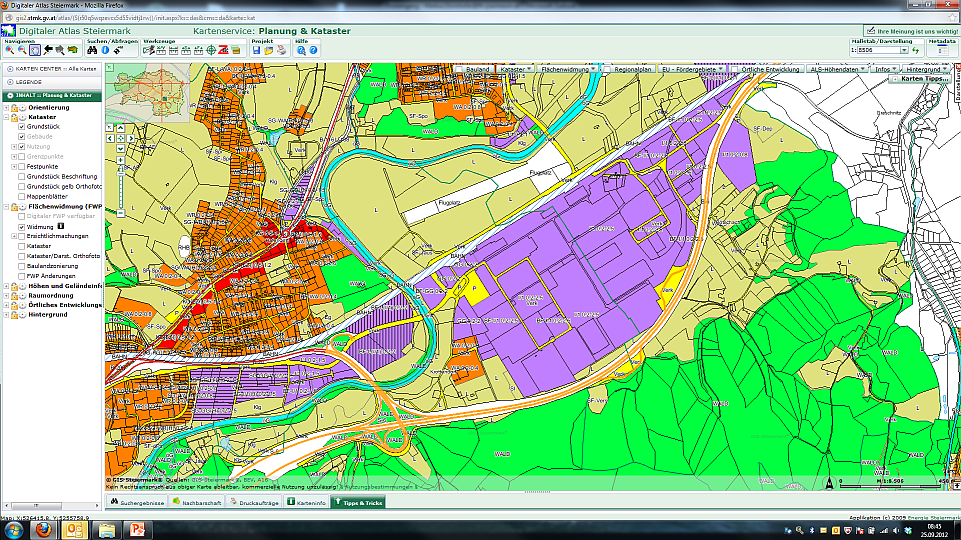
\includegraphics[scale=2.0]{gis-steiermark-kl}
\caption{Zonen}
\end{figure}

\section{Biologie - Populationen}
\begin{figure}[h]
\centering
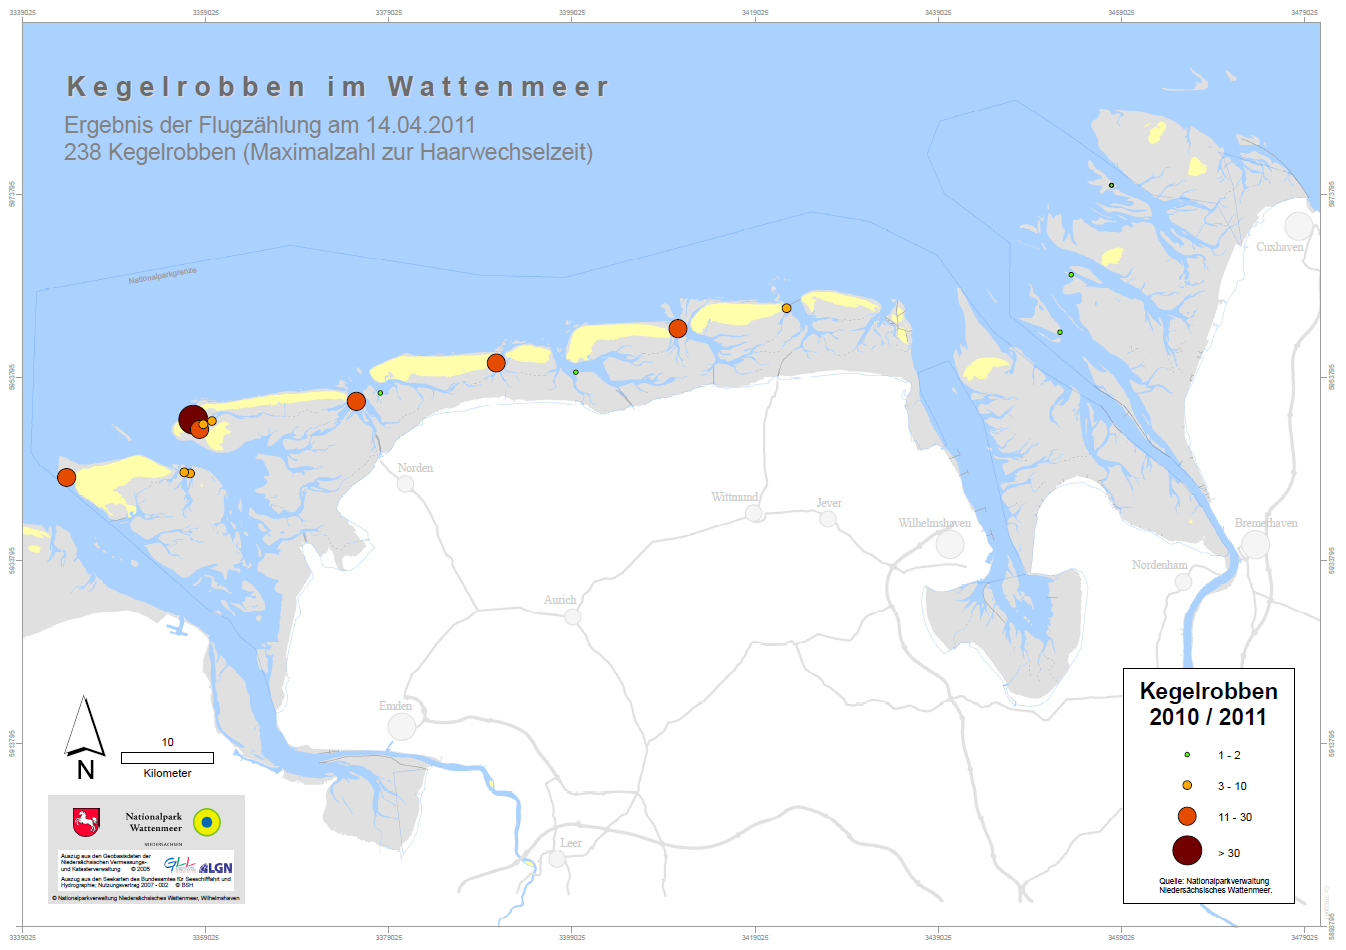
\includegraphics[scale=0.4]{kegelrobben-2011}
\caption{Kegelrobben}
\end{figure}

\section{Navigation}
\begin{figure}[h]
\centering
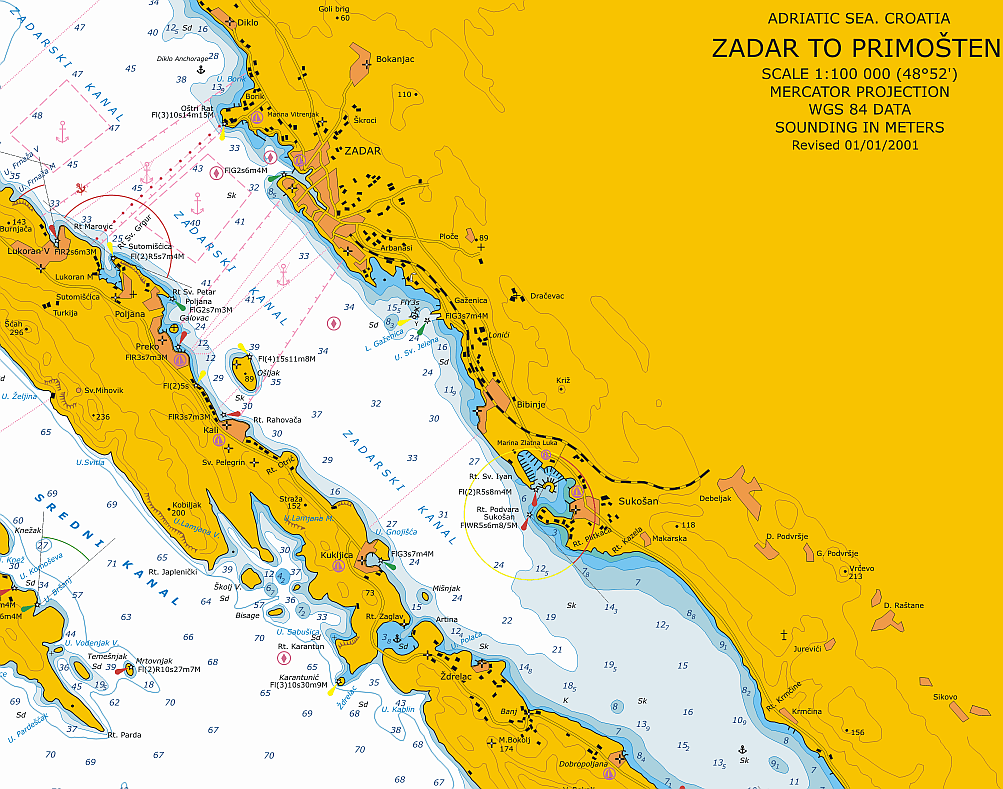
\includegraphics[scale=1.0]{biograd2-small-1000px}
\caption{Seekarte}
\end{figure}

\section{Bev\"olkerungsver\"anderung in der Steiermark}
\begin{figure}[h]
\centering
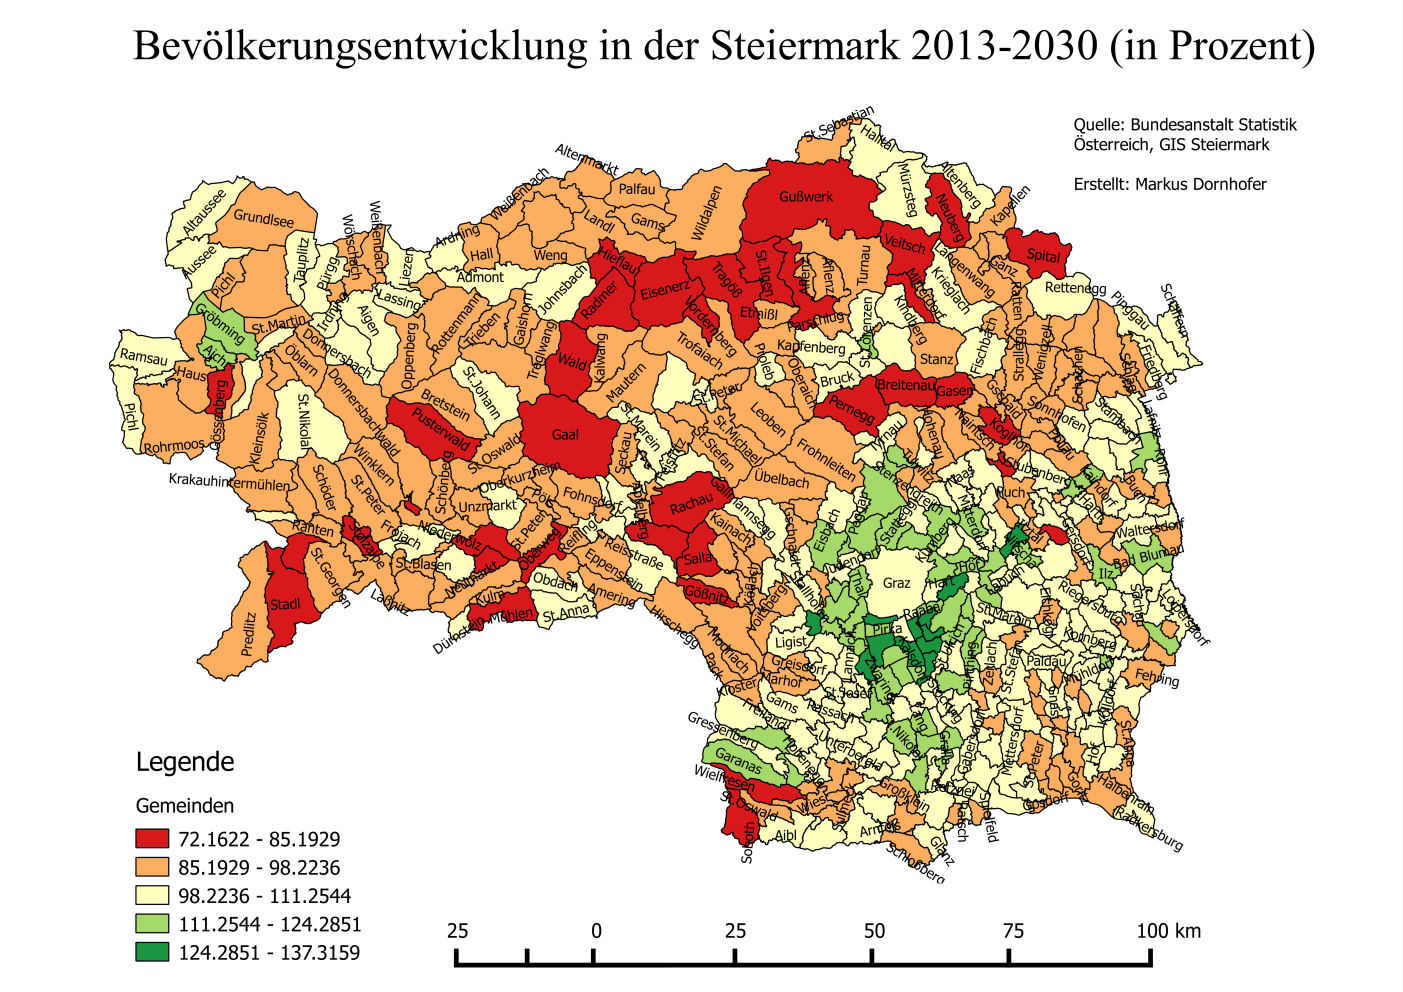
\includegraphics[scale=2.0]{stmk-bev13-30-kl}
\caption{Bev\"olkerungsver\"anderung in der Steiermark}
\end{figure}

\chapter{Geschichte}

\section{1854: Cholera Epidemie}
Im Jahre 1854 gab es in London (Stadtteil Soho) eine Cholera Epidemie. Dr. Snow konnte mit Hilfe einer Aufzeichnung der toten Personen auf den betroffenen Brunnen schlie{\ss}en und damit die Epidemie eind\"ammen.

\begin{figure}[h]
\centering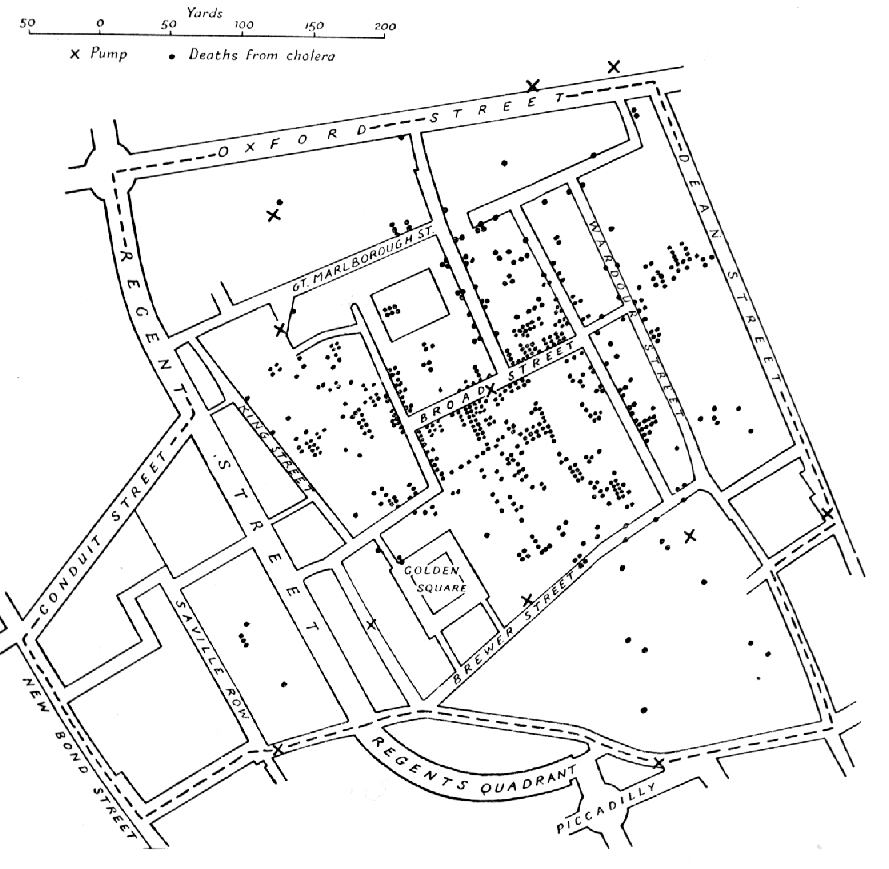
\includegraphics[scale=1.0]{Snow-cholera-map}
\caption{London - Cholera Karte}
\end{figure}

\section{1962: Canadian Geographic Information System}
Die kanadische Regierung suchte nach einen Verwaltungstool ihrer riesigen Waldfl\"achen und schuff damit einen Vorl\"aufer moderner GIS Systeme auf EDV Basis. 

%----------------------------------------------------------------------------------------
%	CHAPTER INTRO
%----------------------------------------------------------------------------------------

\chapterimage{contour_wms_preview_800x400} % Chapter heading image

\chapter{Position und Projektion}

\section{Position}
Grunds\"atzlich kann jede Position auf der Erde mit 2 verschiedenen Winkeln angegeben werden. Die Latidute ist der Winkel vom Aquator zu den Polen. 
Ein Breitengrad ist ein Kreis mit gleicher Latidute. Die Breidengrade werden zu den Polen hin kleiner. Der Bereich der Latidute geht von + 90 Grad zu - 90 Grad. \\
Die Longiduten (Meridiane) haben immer die gleiche L\"ange und verlaufen durch beide Pole. Somit hat ein Grad-Minute  = Seemeile = 1.8 km auf einer Longidute immer die gleiche L\"ange. Der Nullmeridian is willk\"uhrlich gew\"ahlt und geht durch den Stadtteil Greenwich in London. Der Bereich der Lonidute geht von -180 bis +180 Grad. \\
Statt dem Vorzeichen wird oft auch die Himmelsrichtung (z.B. 47°30`N) verwendet.   
 
 
\begin{figure}
        \centering
        \begin{subfigure}[h]{0.2\textwidth}
                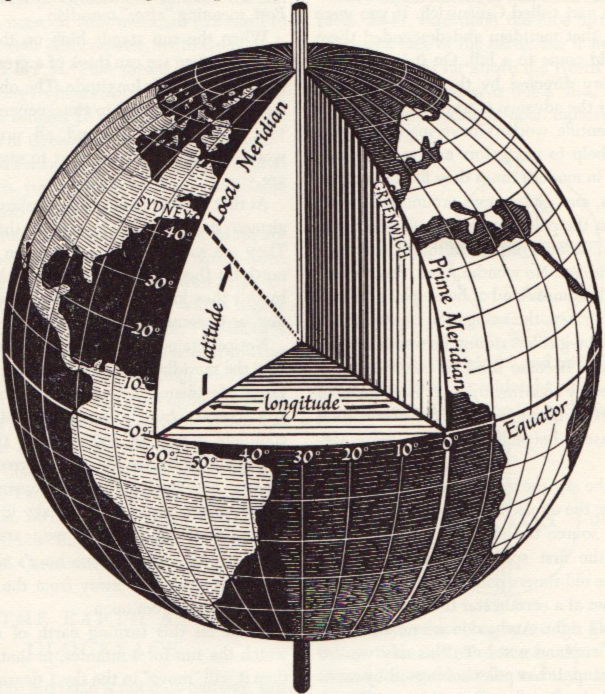
\includegraphics[width=\textwidth]{lat_long_globe}
                \caption{A gull}
                \label{fig:gull}
        \end{subfigure}
     
        \begin{subfigure}[h]{0.2\textwidth}
                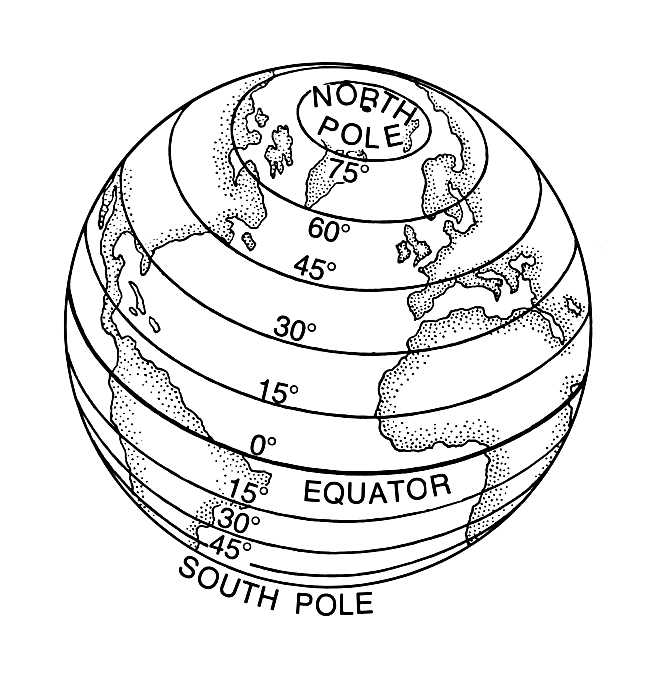
\includegraphics[width=\textwidth]{Latitude_kl}
                \caption{A tiger}
                \label{fig:tiger}
        \end{subfigure}
      
        \begin{subfigure}[h]{0.2\textwidth}
                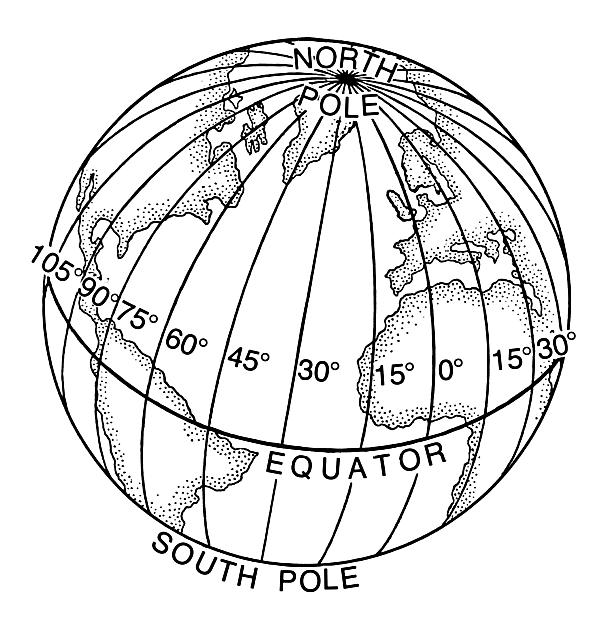
\includegraphics[width=\textwidth]{Longitude_kl}
                \caption{A mouse}
                \label{fig:mouse}
        \end{subfigure}
        \caption{Pictures of animals}\label{fig:animals}
\end{figure} 

\section{Umwandlung von Dezimalgrad in Gradminuten und Gradsekunden}

$lat=47.256$

$lat_min=0.256*60=15.36$

$lat_sek=0.36*60=21.6$

\begin{figure}[h]
\centering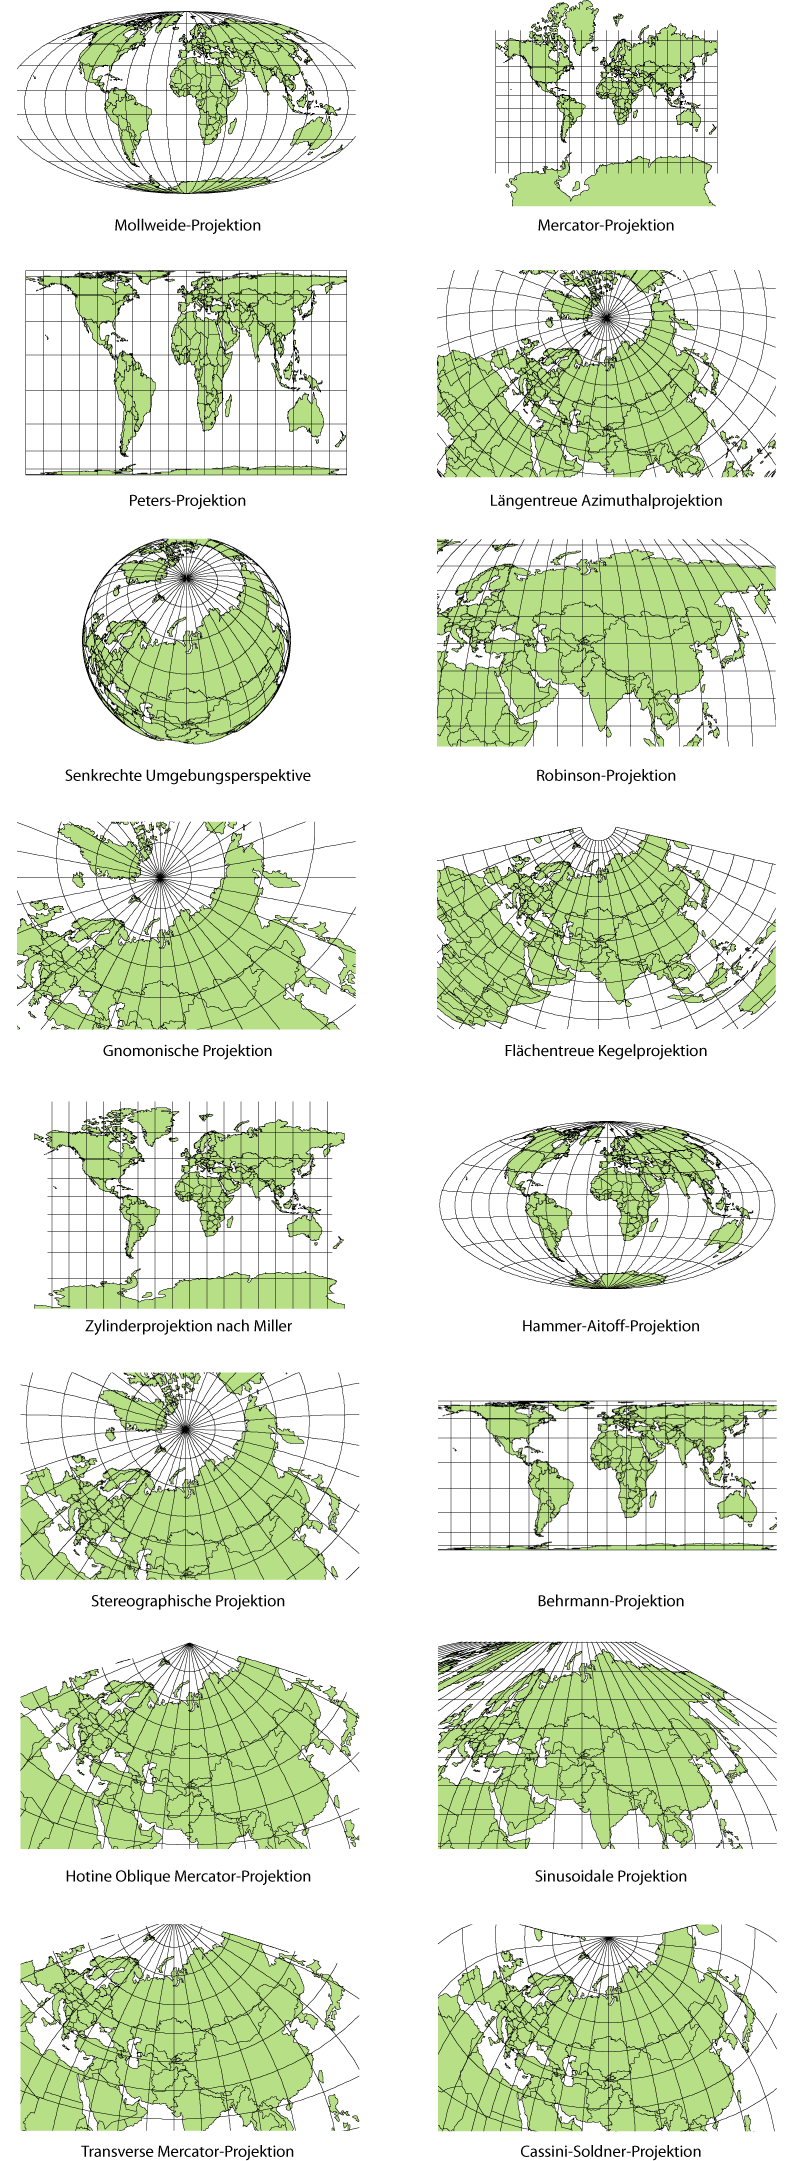
\includegraphics[scale=0.5]{Netzentwuerfe-Kartenprojektionen}
\caption{Shapefile}
\end{figure}

%----------------------------------------------------------------------------------------
%	CHAPTER GEODATA
%----------------------------------------------------------------------------------------


\chapter{Geodaten}
Geodaten sind Informationen die einen Punkt auf der Erde zugewiesen sind. Sie enthalten auch eine r\"aumliche Information.
\section{Raster und Vektordaten}\index{RasterundVektordaten}

\begin{figure}[h]
\centering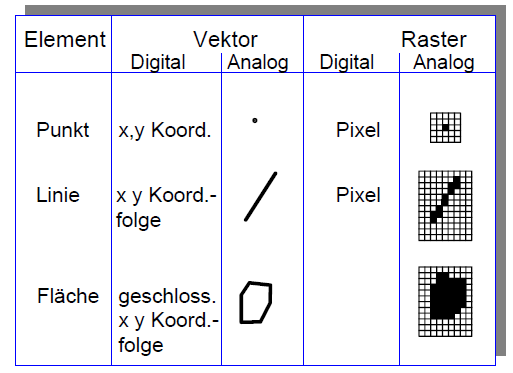
\includegraphics[scale=0.6]{vector-raster}
\caption{Shapefile}
\end{figure}

\subsection{Rasterdaten}

Rasterdaten sind zum Beispiel:
\begin{itemize}
\item Orthofotos
\item Luftaufnahmen mit Radar oder Laser (z.B. SRTM)
\item Eingescannte Karten (z.B. historische Karten)
\end{itemize}

\subsection{Vektordaten}

Vektordaten werden eingesetzt bei:
\begin{itemize}
\item Navigation
\item Kartendienste
\item OpenStreetMap
\end{itemize}

Vektordaten können mit einem Quantisierungsverlust in ein Rasterbild umgewandelt werden. Bei OpenstreetMap werden die Vektordaten kontinuierlich in neuen Kartenkacheln (Siehe WMTS)
umgewandelt. \\
Oft m\"ochte man durch eine Umwandlung auch die Originalvektordaten sch\"utzen und nur Zugriff auf die Rasterdaten zulassen.   


%----------------------------------------------------------------------------------------
%	CHAPTER DATA FORMAT
%----------------------------------------------------------------------------------------

\chapter{Datenformate}
\section{Dateien}\index{Dateien}
Dateien k\"onnen lokal auf dem PC verwaltet werden. Ein gemeinsames Bearbeiten der Dateien ist schwierig. Wird die Datenmenge sehr gro{\ss} kann es auch zu Problemen f\"uhren. Bei den meisten Personen sind Files jedoch noch immer sehr beliebt.
\subsection{Shapefiles (SHP)}
Geodaten werden in Shapefiles gespeichert und k\"onnen dort mit Sachdaten verkn\"upft werden.  Das format wurde von der Firma ESRI (ArcGIS) entwickelt und kann aber auch von anderen Programmen verabeitet werden.
\begin{figure}[h]
\centering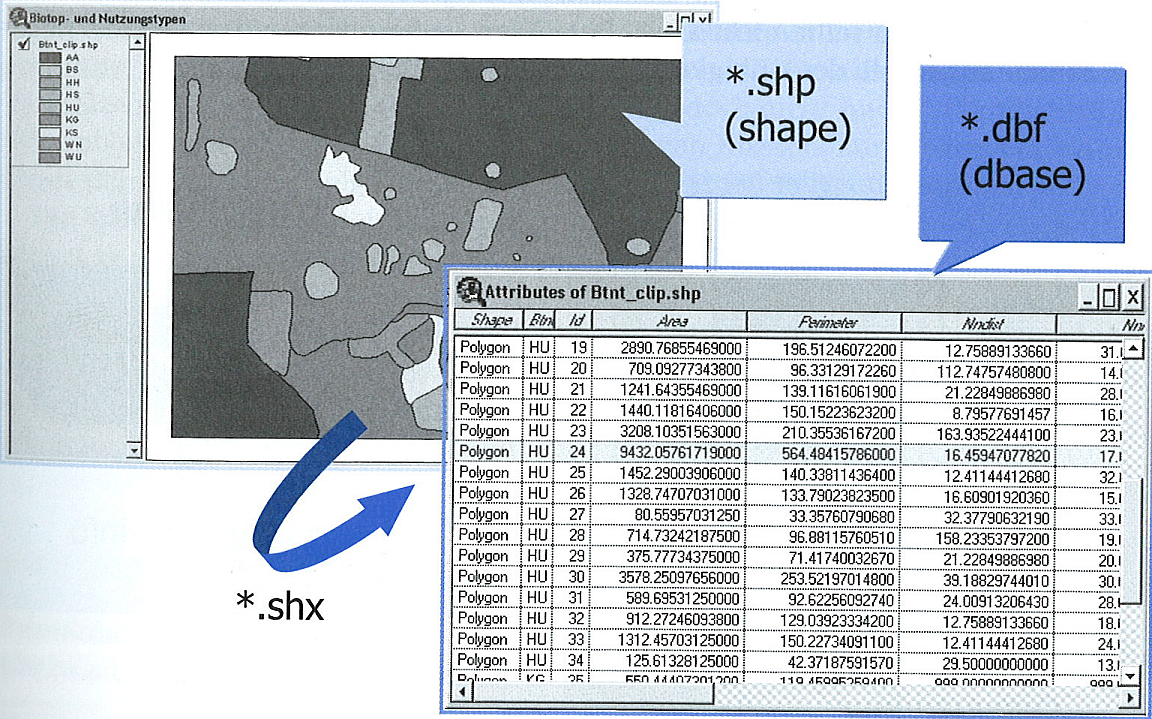
\includegraphics[scale=2.0]{esri-daten-format_kl}
\caption{Shapefile}
\end{figure}


\subsection{H\"ohen-Dateien (HGT/SRTM)}
Hier handelt es sich um ein Rasterformat mit H\"oheninformation. Statt einen Farbwert ist hier f\"ur jedes Pixel ein H\"ohenwert gespeichert. Meist wurden dabei mit einem Radarger\"at die H\"ohe von einem Spaceshuttle vermessen(Shuttle Radar Topography Mission). 
\begin{figure}[h]
\centering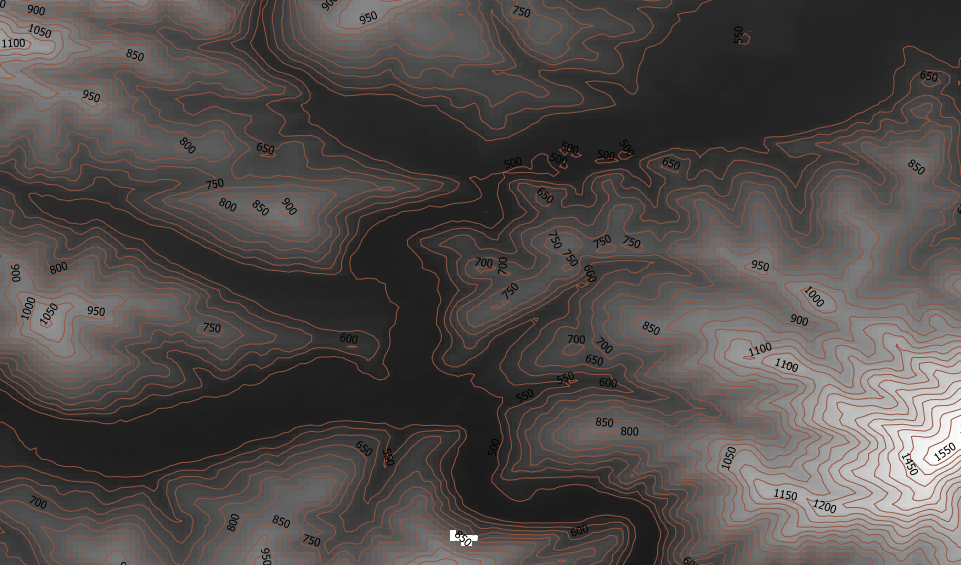
\includegraphics[scale=0.5]{contour_preview}
\caption{H\"ohenschichtlinien}
\end{figure}


\subsection{GeoTiff}
GeoTiff ist ein Bild, da{\ss} mit mehreren Punkten auf der Erde referenziert wird. Damit kann es mit anderen Geodaten dargestellt werden. Mit den Bilder kann auch offline gearbeitet werden und eignen sich besonders f\"ur kleine Bereiche. 

\section{Geodatenbank}\index{Geodatenbank}
Datenbanken bitten auch viele M\"oglichkeiten im GIS Bereich. Unter den vorhanden M\"oglichkeiten wie Zugangberechtigungen, Multiuser und Datenauswahl, gibt es auch Möglichkeiten der r\"aumlichen Analyse in der Datenbank. 

\subsection{POSTGIS}
F\"ur die freie Postgres Datenbank wurde die Erweiterung Postgis entwickelt. Damit sind auch r\"aumliche Analysen oder Abfragen in der Datenbank m\"oglich. Z.B. K\"onnten alle Lebensmittelgesch\"afte im Umkreis von 1 km abgefragt werden. Oder Zeige mir alle Gemeinegrenzen an.    
\begin{figure}[h]
\centering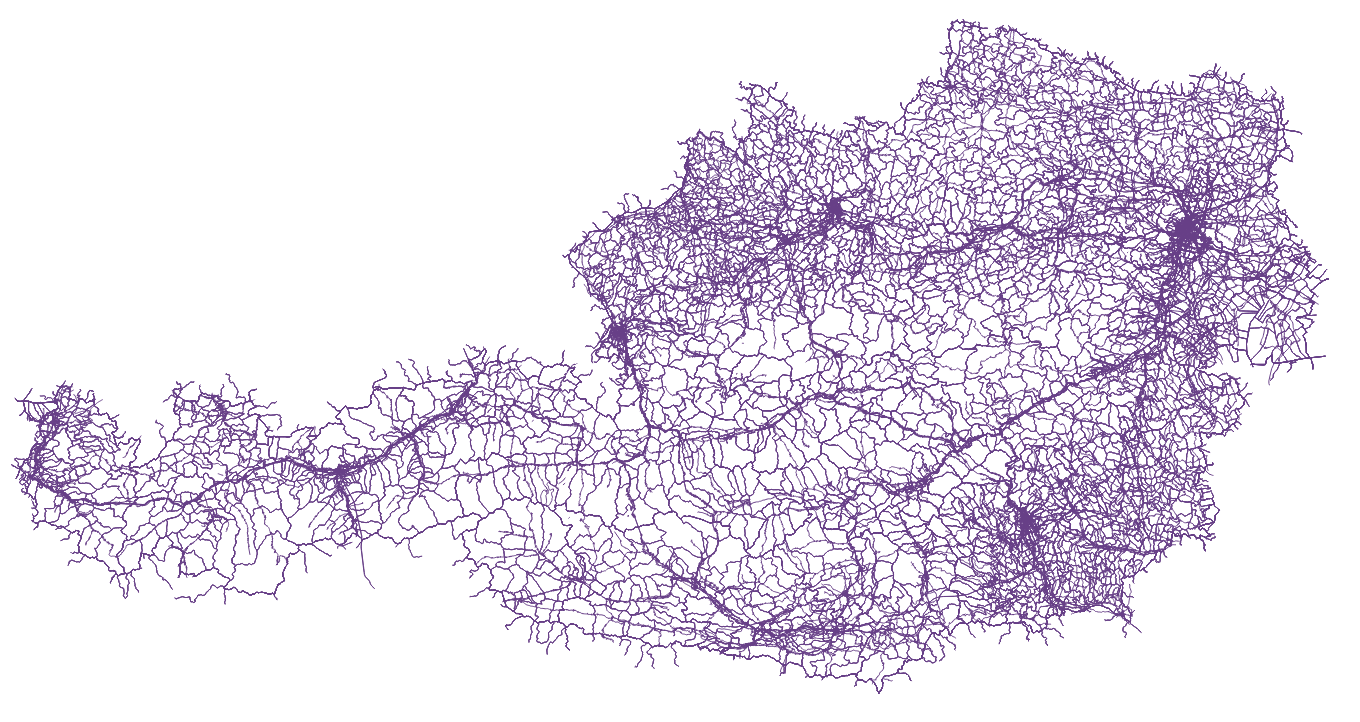
\includegraphics[scale=0.5]{postgis_ohne_stil}
\caption{OSM Daten in POSTGIS ohne Stil}
\end{figure}
Die Videos von Paul Ramsey dem Mitgr\"under von Postgis sind zu empfehlen. \url{http://blog.cleverelephant.ca/}

\section{Webdienste}\index{Webdienste}
F\"ur die Abfrage eines Webdienstes ist eine Verbindung zum Server (Online) notwendig. \"Uber eine URL kann einen genauere Beschreibung zum Webservice abgerufen werden. Das wird von der GIS Software automatisch gemacht, man muss nur die URL als Verbindungsparameter angeben. In den Einstellungen sind die Möglichkeiten der Projektionen, Darstellungsbereiche und Bildformate genau definiert. 
\begin{figure}[h]
\centering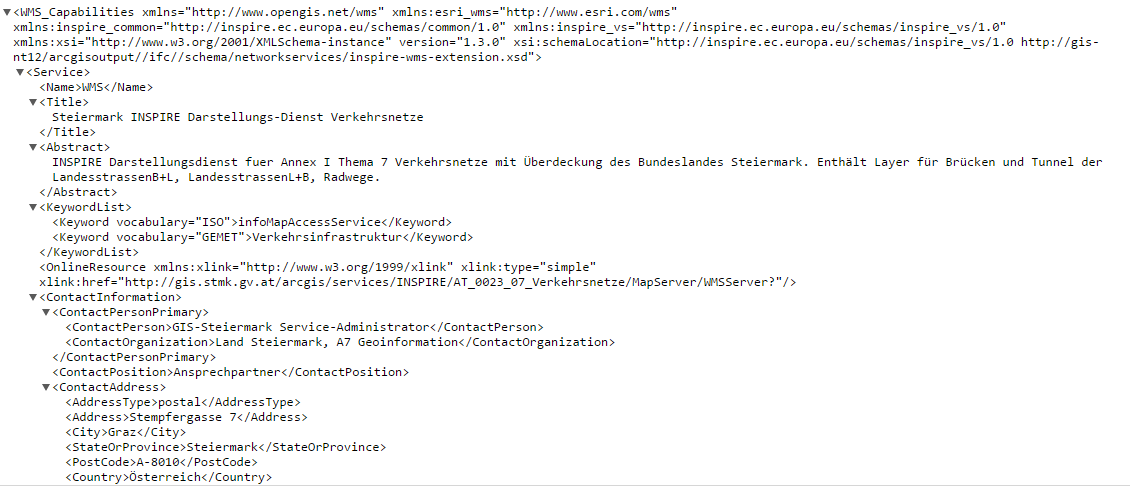
\includegraphics[scale=0.5]{xml_request}
\caption{XML Definition}
\end{figure}
\subsection{Web Map Service (WMS)}
Hier werden Rasterkarten für einen bestimmten Bereich und in einer bestimmten Projektion heruntergeladen. Beim Verschieben der Karte muss jedoch immer ein neues Bild geladen werden (langsam)  Z.B. Orthofotos, Laserscans, Verkehrsstra{\ss}en, ...


\subsection{Web Map Tile Service (WMTS)}
Als Erweiterung zum WMS wird hier die Karte in Kacheln (Tiles) zu einer fixen Anzahl von Pixel (z.B. 256x256) aufgeteilt. Dadurch muss nicht das gesamte Bild bei einer Verschiebung nachgeladen werden sondern nur die neuen Kacheln (schneller) 


\subsection{Web Feature Service (WFS)}
Hier k\"onnen auch Vektorlayer \"uber ein Webservice verteilt werden.
\footnote{Zus\"atzliche Information}


\chapterimage{Osm-heatmap_1320x860} % Chapter heading image
\chapter{Datenquellen}
In der Vergangenheit war der Erwerb von Geodaten die häufigste Quelle. In den letzten Jahren hat sich viel ver\"andert. Durch Community Projekte, wie zum Beispiel OpenStreetMap werden nun viele Daten auf freiwilliger Basis erhoben. Auch Beh\"orden neigen nun dazu, dass sie Geodaten die mit \"offentlichen Geldern finanziert wurden zur Verf\"ugung stellen. Zu guter letzt ist auch durch das Smartphone die Erhebung von Daten deutlich erleichtert worden.
\section{OpenStreetMap(2004)}

\begin{figure}[h]
\centering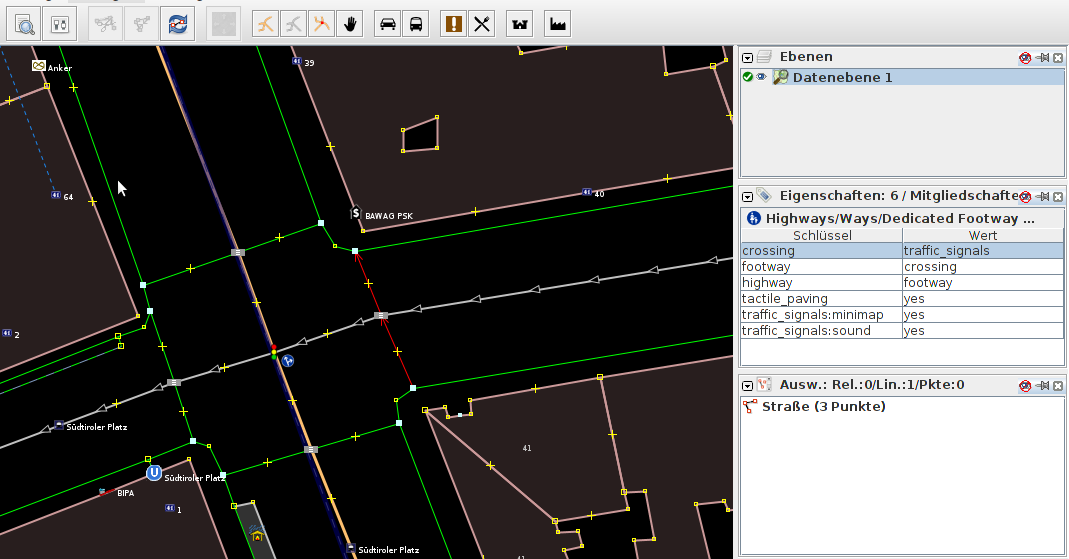
\includegraphics[scale=0.5]{jsom_kl}
\caption{OSM Editor}
\end{figure}

\section{OpenData(2010)}
Unter den Begriff OpenData sind meist beh\"ordliche Daten gemeint. Ein kleiner Teil ist auch als Geodaten verf\"ugbar oder kann zuminderst mir Geodaten verkn\"upft werden (Siehe Bev\"olkerungsentwicklung). \url{http://data.gv.at/} 
\subsection{GIS Steiermark}
Alle Bundesl\"ander stellen allgemeine Geodaten zur Verf\"ugung. So werden vom Land Steiermark  Shapefiles der Bezirksgrenzen, der Orte, der Gemeinden, des Hauptgew\"asser und der Hauptstra{\ss}en zum Download bereitgestellt. \url{http://www.gis.steiermark.at/cms/ziel/14292094/DE/} 

\subsection{Vogis Voralberg}
In \"Osterreich wird die gr\"o{\ss}te Vielfalt von Daten vom Land Vorarlberg zur Verf\"ugung gestellt. Das liegt wahrscheinlich an der n\"ahe zur Schweiz, die auch eine gro{\ss}e GIS Geschichte hat. \\
Das Land Vorarlberg ist auch ein finanzieller Unterst\"utzer des QGIS Projektes. \url{http://vorarlberg.at/vorarlberg/bauen_wohnen/bauen/vermessung_geoinformation/start.htm}
\subsection{Verwaltungsgrundkarte - basemap (2012)}
In \"Osterreich wurde eine einheitliche Verwaltungskarte der \"Offentlichkeit zug\"anglich gemacht. Sie beruht auf einen Graphenintegrationsplatform (GIP). Damit kann auch ein einheitliche Routingabfrage (z.B. Verwendung bei Pendlerrechner) erm\"oglicht werden. 
\begin{figure}[h]
\centering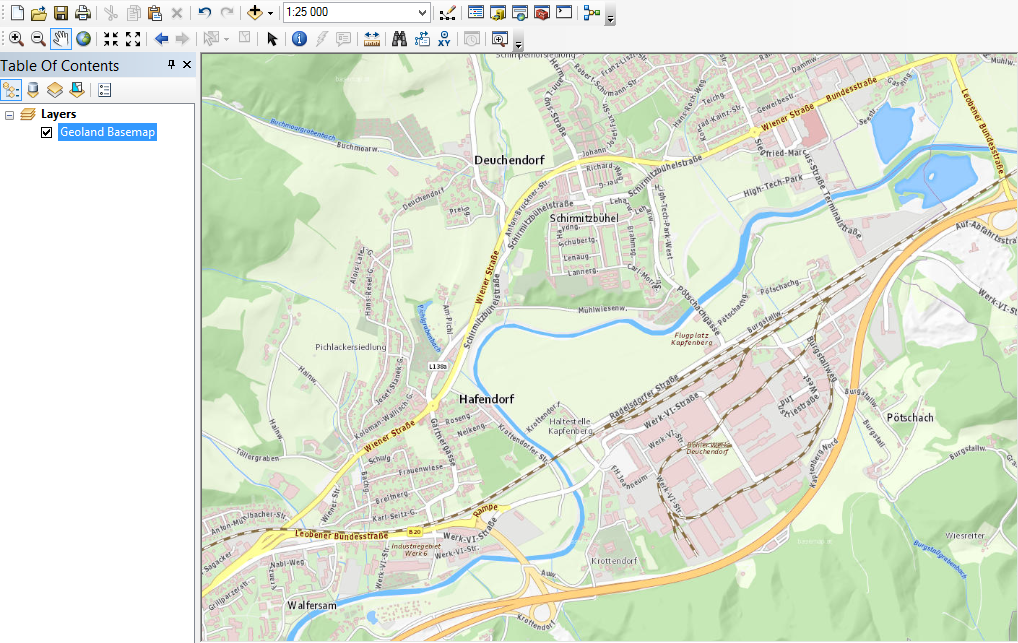
\includegraphics[scale=0.5]{arcmap_basemap}
\caption{Basemap (WMTS)}
\end{figure}



\section{Eigene Daten}
Zur Erhebung eigener Daten werden meist Orthofotos oder mobile GPS Ger\"ate verwendet. F\"ur Smartphones gibt es Applikationen, womit Wege mit zus\"atzlichen Informationen (z.B. Sprachnachrichten, Fotos oder Textmeldungen) aufgezeichnet werden k\"onnen.  \\
Die Erhebung eigener Geodaten ist sehr zeitintensiv und stellt einen gro{\ss}en Kostenfaktor dar.


\begin{figure}[h]
\centering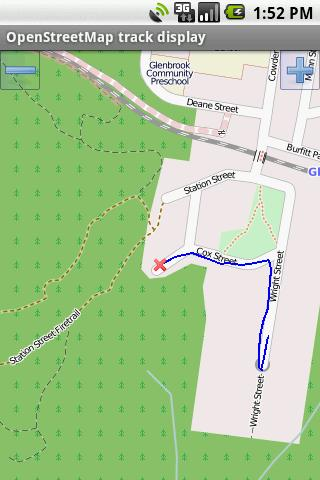
\includegraphics[scale=0.6]{osm_tracker}
\caption{OSM Editor}
\end{figure}

\chapter{Werkzeuge}
\section{ArcGIS}\index{ArcGIS}
Die kommerzielle L\"osung der Firma ESRI hat den Namen ArcGIS. Dieses Produkt wird sehr h\"aufig bei Beh\"orden eingesetzt und hat auch seinen Preis. 
\section{QGIS}
QGIS ist eine OpenSource L\"osung die sehr aktiv entwickelt wird. Weitere OpenSource Projekte (z.B. GRASS GIS) werden von QGIS eingebunden. 
Die Schnittstelle ist sehr bedienerfreundlich und alle 4 Monate wird eine neue Version ver\"offentlicht.
\\
Die \"Osterreicherin Anita Grasser vom AIT sitzt im Steering Komitee vom QGIS Projekt.
\url{http://anitagraser.com/}
\section{OSGeo}
Unter dem Namen OSGeo wird ein Betriebssystem auf Linuxbasis vermarktet. Die Software ist kostenfrei und enth\"alt zahlreiche GIS Pakete.



%----------------------------------------------------------------------------------------
%	BIBLIOGRAPHY
%----------------------------------------------------------------------------------------

\chapter*{Bibliography}
\addcontentsline{toc}{chapter}{\textcolor{ocre}{Bibliography}}
\section*{Books}
\addcontentsline{toc}{section}{Books}
\printbibliography[heading=bibempty,type=book]
\section*{Articles}
\addcontentsline{toc}{section}{Articles}
\printbibliography[heading=bibempty,type=article]

%----------------------------------------------------------------------------------------
%	INDEX
%----------------------------------------------------------------------------------------

\cleardoublepage
\phantomsection
\setlength{\columnsep}{0.75cm}
\addcontentsline{toc}{chapter}{\textcolor{ocre}{Index}}
\printindex

%----------------------------------------------------------------------------------------

\end{document}